\chapter{Algorithms and Indices}

\section{Sorting Algorithms}
\subsection{Quicksort}
\subsection{Merge Sort}
\subsection{Tim Sort}
\subsection{Radix Sort}
\subsection{Top-N with Heaps}

\unfinished

\section{Joins}
\subsection{Database Normalisation}
% Normal Forms
\unfinished

\subsection{Join Types}
Normalised databases naturally require joins to re-compose data.

\begin{examplebox}{We would be honoured if you would join us\dots}
    Provide some examples of types of queries that would require a join.
    \tcblower
    \unfinished
\end{examplebox}

\begin{definitionbox}{Join}
    A join is a cross product with selection using data from both relations ($\sigma_{p(R_A.x, R_B.y)} (R_A \times R_B)$).
\end{definitionbox}

\subsubsection{Inner Joins}
\begin{tcbraster}[raster columns=2, raster equal height]
    \begin{definitionbox}{Inner Join}
        A join only returning rows from both tables which satisfy a predicate/condition.
        \begin{center}
            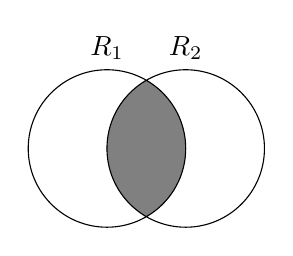
\begin{tikzpicture}[fill=gray]
                % left hand
                \scope
                \clip (1,0) circle (1);
                \fill (0,0) circle (1);
                \endscope
                % right hand
                \scope
                \clip (0,0) circle (1);
                \fill (1,0) circle (1);
                \endscope
                % outline
                \draw (0,0) circle (1) (0,1)  node [text=black,above] {$R_1$}
                      (1,0) circle (1) (1,1)  node [text=black,above] {$R_2$};
            \end{tikzpicture}
        \end{center}
    \end{definitionbox}
    \begin{definitionbox}{Natural Join}
        Joining two tables with an implicit join clause (join on equality on a column present in both tables
        \[R_1 \bowtie R_2\]
        \begin{minted}{sql}
FROM R1 NATURAL JOIN R2
FROM R1 JOIN R2 USING(id)
        \end{minted}
    \end{definitionbox}
\end{tcbraster}
\begin{tcbraster}[raster columns=2, raster equal height]
    \begin{definitionbox}{Theta Join}
        Joining two tables based on a condition/predicate $\theta$.
        \[R_1 \overset{\theta}{\bowtie} R_2\]
        \begin{minted}{sql}
FROM R1, R2 WHERE theta(R1, R2)
FROM R1 JOIN R2 ON theta(R1, R2)
        \end{minted}
    \end{definitionbox}
    \begin{definitionbox}{Equi Join}
        A \textbf{theta join} with a single equivalence condition. A \textbf{natural join} is an implicit \textbf{equi join}.
        \[R_1 \bowtie_{R_1.x = R_2.x}\]
        \begin{minted}{sql}
FROM R1, R2 WHERE R1.x = R2.x
        \end{minted}
    \end{definitionbox}
\end{tcbraster}
\begin{tcbraster}[raster columns=2, raster equal height]
    \begin{definitionbox}{Cross Join}
        Just cartesian product with no selection.
        \[R_1 \times R_2\]
        \begin{minted}{sql}
    FROM R1, R2
    FROM R1 CROSS JOIN R2
        \end{minted}
    \end{definitionbox}
    \begin{definitionbox}{Anti Join}
        A \textbf{theta join} using an inequality predicate
        \[R_1 \bowtie_{R_1.x <> R_2.x} R_2\]
        \begin{minted}{sql}
FROM R1 JOIN R2 ON R1.x <> R2.x
        \end{minted}
    \end{definitionbox}
\end{tcbraster}

\subsubsection{Outer Joins}
\begin{tcbraster}[raster columns=2, raster equal height]
    \begin{definitionbox}{Left Join}
        \[R_1 \overset{L}{\bowtie} R_2\]
        Returns all rows of $R_1$ even if no rows in $R_2$ match (in which case columns are \mintinline{sql}{NULL}).
        
            \begin{center}
                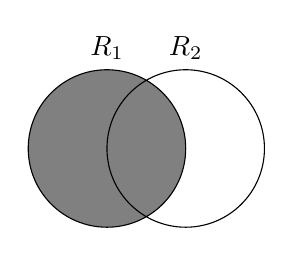
\begin{tikzpicture}[fill=gray]
                    % left hand
                    \scope
                    \fill (0,0) circle (1);
                    \endscope
                    % right hand
                    \scope
                    \clip (0,0) circle (1);
                    \fill (1,0) circle (1);
                    \endscope
                    % outline
                    \draw (0,0) circle (1) (0,1)  node [text=black,above] {$R_1$}
                            (1,0) circle (1) (1,1)  node [text=black,above] {$R_2$};
                \end{tikzpicture}
            \end{center}
            \begin{minted}{sql}
FROM R1 LEFT JOIN R2 ON ... 
            \end{minted}
    \end{definitionbox}
    \begin{definitionbox}{Right Join}
        \[R_1 \overset{R}{\bowtie} R_2\]
        Returns all rows of $R_2$ even if no rows in $R_1$ match (in which case columns are \mintinline{sql}{NULL}).
            \begin{center}
                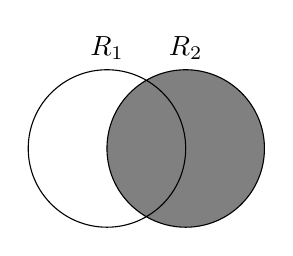
\begin{tikzpicture}[fill=gray]
                    % left hand
                    \scope
                    \clip (1,0) circle (1);
                    \fill (0,0) circle (1);
                    \endscope
                    % right hand
                    \scope
                    \fill (1,0) circle (1);
                    \endscope
                    % outline
                    \draw (0,0) circle (1) (0,1)  node [text=black,above] {$R_1$}
                            (1,0) circle (1) (1,1)  node [text=black,above] {$R_2$};
                \end{tikzpicture}
            \end{center}
            \begin{minted}{sql}
FROM R1 RIGHT JOIN R2 ON ... 
            \end{minted}
    \end{definitionbox}
\end{tcbraster}
\begin{definitionbox}{Full Outer Join}
    \[R_1 \overset{O}{\bowtie} R_2 \equiv R_1 \overset{L}{\bowtie} R_2 \cup R_1 \overset{R}{\bowtie} R_2\]
    Returns all rows from all tables matching, with rows from either $R_1$ or $R_2$ that do not have match associated with \mintinline{sql}{NULL} columns from the other table.
    \begin{center}
        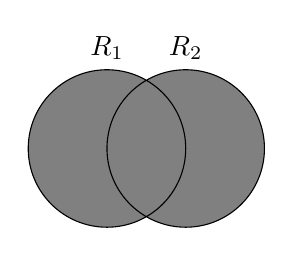
\begin{tikzpicture}[fill=gray]
            % left hand
            \scope
            \fill (0,0) circle (1);
            \endscope
            % right hand
            \scope
            \fill (1,0) circle (1);
            \endscope
            % outline
            \draw (0,0) circle (1) (0,1)  node [text=black,above] {$R_1$}
                    (1,0) circle (1) (1,1)  node [text=black,above] {$R_2$};
        \end{tikzpicture}
    \end{center}
    \begin{minted}{sql}
FROM R1 FULL OUTER JOIN R2 ON ... 
FROM R1 FULL JOIN R2 ON ... 
FROM (SELECT * FROM R1 LEFT JOIN R2 ON ... UNION SELECT * FROM R1 RIGHT JOIN R2 ON ...)
    \end{minted}
\end{definitionbox}


\begin{examplebox}{Which imposter?}
    Which of the following are joins?
    \begin{multicols}{2}
    \begin{enumerate}
        \item {
\begin{minted}{sql}
SELECT R.r, S.s
FROM R, S
WHERE R.id = S.id;
\end{minted}
}
\item {
    \begin{minted}{sql}
SELECT R.r, S.s
FROM R, S
WHERE R.r = R.id
    \end{minted}
}
        \item {
        \begin{minted}{sql}
SELECT R.r
FROM R, S
WHERE R.id = S.id;
        \end{minted}
        }
        \item {
            \begin{minted}{sql}
SELECT R.r
FROM R, S
WHERE R.r = "some string";
            \end{minted}
        }
    \end{enumerate}
    \end{multicols}
    \tcblower
    \begin{enumerate}
        \item \textbf{Join} (Selects on both $R$ and $S$)
        \item \textbf{Not a Join} (Only selects on $R$)
        \item \textbf{Join} (The $\sigma$ selection is on $R$ and $S$, so a join even if only $R$ is projected)
        \item \textbf{Not a Join} (Only selects on $R$)
    \end{enumerate}
\end{examplebox}

\subsection{Nested Loop Join}
We can implement a basic join naively using nested loops.
\begin{minted}{Cpp}
#include <tuple>
#include <vector>

using namespace std;

template <typename... types> using Table = vector<tuple<types...>>;

template <size_t leftCol, size_t rightCol, typename... TypesOne, typename... TypesTwo>
Table<TypesOne..., TypesTwo...> nest_loop_join(Table<TypesOne...> &left, Table<TypesTwo...> &right) {
  Table<TypesOne..., TypesTwo...> result;
  for (auto &leftElem : left) for (auto &rightElem : right) {
    if (get<leftCol>(leftElem) == get<rightCol>(rightElem)) {
      result.push_back(tuple_cat(leftElem, rightElem));
    }
  }
  return result;
}
\end{minted}
\[\text{Time Complexity} = \begin{cases}
    \cfrac{\Theta (|left| \times |right|) }{2} & \text{ If elements unique} \\
    \Theta (|left| \times |right|)  & otherwise \\
\end{cases}\]
\begin{tabbox}{prosbox}
    \textbf{Simple} & Easy to reason about (memory accesses \& complexity) \\
    \textbf{Trivially Parallel} & Loop iterations are not dependent, so can be parallelised. \\
    \textbf{Sequential I/O} & Access is done in the order of the tables storage (sequential access better for both memory \& disk) \\
\end{tabbox}
\begin{tabbox}{consbox}
    \textbf{Performance} & Linear time complexity. \\
\end{tabbox}

\subsection{Sort Merge Join}
If we assume both tables are sorted, and values (being joined on) are unique.
\begin{itemize}
  \item Two cursors (one per table)
  \item Advance cursors in order, if the value on the left exceeds the right there can be no joins for the left row (and vice versa).
\end{itemize}
\begin{minted}{cpp}
template <size_t leftCol, size_t rightCol, typename... TypesOne, typename... TypesTwo>
Table<TypesOne..., TypesTwo...> sort_merge_join(Table<TypesOne...> &left, Table<TypesTwo...> &right) {
  Table<TypesOne..., TypesTwo...> result;

  auto leftIndex = 0;
  auto rightIndex = 0;

  while (leftIndex < left.size() && rightIndex < right.size()) {
    auto leftElem = left[leftIndex];
    auto rightElem = left[rightIndex];

    if (get<leftCol>(leftElem) < get<rightCol>(rightElem)) {
      leftIndex++;
    } else if (get<leftCol>(leftElem) > get<rightCol>(rightElem)) {
      rightIndex++;
    } else {
      result.push_back(tuple_cat(leftElem, rightElem));
      leftIndex++;
      rightIndex++;
    }
  }

  return result;
}
\end{minted}
\[\text{Time Complexity} = \]
\unfinished